% !TeX root = ../template-UNAMFC.tex
\section{Estructuras útiles}
%----------------------------------------------------------------------------------
\begin{frame}{\underline{¿Ventajas de esta plantilla?}} % De esta forma se pone el subrayado
	{No se reescala nada}
	\centering
	\begin{columns}
		\column{.9\squeezethree}
		Se debe copmpilar en \emphb{Xelatex} y tener instalado Gotham en las fuentes del sistema
		{\fontseries{l}\titlefont\selectfont Algo así}
		{\titlefont Algo así}
		\begin{itemize}
			\item El aspectratio es 16:9
			\item El tamaño de la hoja no es el de beamer pero permite lo siguiente:
			\begin{itemize}
				\item La letra defalt es 11pt
				\item Reecalado sin deformar la imagen
				\begin{itemize}
					\item Ni las ecuaciones se hacen feas
					\item Y gráficas sin escala se ven como la de la derecha
				\end{itemize}
			\end{itemize}
		\end{itemize}
		\vskip3em
		En Latex/setup.tex está el paquete de \emphr{esp-grid}. Si se descomenta se muestran las coordenadas para colocar varios de los elementos en esta plantilla.
		
		\column{1.8\squeezethree} \centering
		Image with scale = 1 with a font of 11pt\\[1em]
		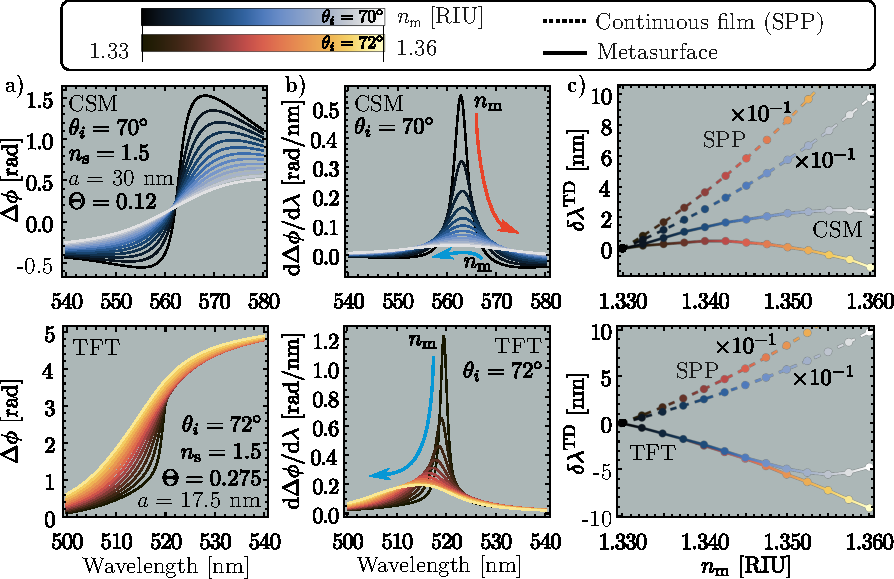
\includegraphics[scale = 1]{img/Fig-Sens.pdf}
	\end{columns}
	
\end{frame}

\section{Ejemplos de algunas diapositivas}
%----------------------------------------------------------------------------------
\begin{frame}[t]{\underline{Ejemplo de una diapositiva para el contexto}}
		{Beamercolorbox y tikz}

	\vskip2em%
	\hskip2em%
	\begin{beamercolorbox}[wd=\squeezethree]{}
		Pones el texto y \emphb{resaltamos algo} \emphr{con dos colores} y un a referencia a mano.\footnotemark[1]\\[1em]
    	
    	Una lista pequeña nada más
        \begin{itemize}  
            \item Parametro 1
			\item El 2
			\item Y el tercero
        \end{itemize}
    \end{beamercolorbox}%
     \begin{textblock*}{40mm}(50mm,60mm)\scriptsize
     	\rule{20mm}{.5pt}\\
    	\footnotemark\fullcite{gonzalez-alcalde_large_2020}
    \end{textblock*}

	
% Nanorods kabashin_plasmonic_2009 -------------------------------
    \begin{textblock*}{1mm}(105mm,20mm)
	\begin{tikzpicture}[font=\scriptsize]
	\node (img) {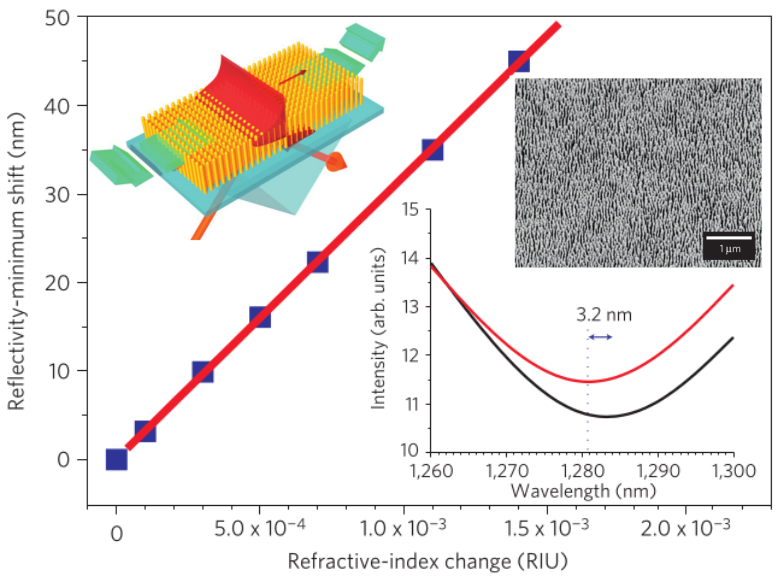
\includegraphics[width = 85mm]{img/1-nanorods.png}};
	\path (img.45) node [anchor = north west, xshift=10mm] {\begin{minipage}{30mm}
			\begin{flushleft}
                \fullcite{kabashin_plasmonic_2009} \\[1em]
				La referencia de la imagen se pone a mano\\[1em]
				Y se coloca relatiava a la imagen grande
			\end{flushleft}
			\end{minipage}};	
	\end{tikzpicture}
    \end{textblock*}



    % COVID qiu_dual_2020 -----------------------------------------
    \begin{textblock*}{1mm}(10mm,85mm)
	\begin{tikzpicture}[font=\scriptsize]
		\node (img) {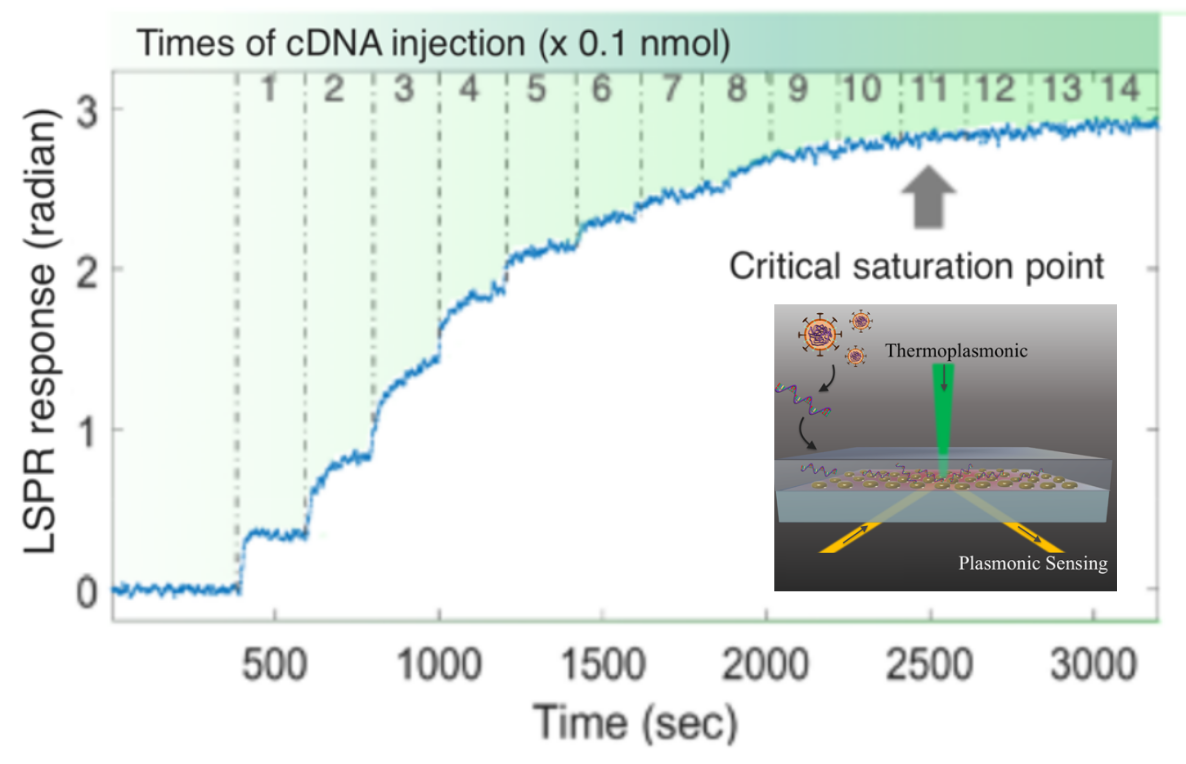
\includegraphics[width = 95mm]{img/1-covid.png}};
		\path (img.0) node [anchor = north west, xshift=-2.5mm] {\begin{minipage}{30mm}
				\begin{flushleft}
				\fullcite{qiu_dual_2020} \\[1em]
				Se usa flushleft\\
				flush   right\\
				Y textblock
				\end{flushleft}
		\end{minipage}};	
	\end{tikzpicture}
	\end{textblock*}


    % Nanodisks svedendahl_refractometric_2014 --------------------
    \begin{textblock*}{1mm}(170mm,65mm)
	\begin{tikzpicture}[font=\scriptsize]
		\node (img) {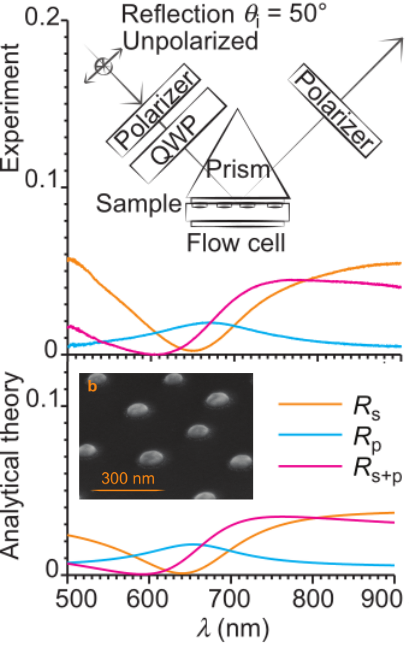
\includegraphics[width = 55mm]{img/1-phase.png}};
		\path (img.180) node [anchor = north east, xshift=0mm] {\begin{minipage}{30mm}
				\begin{flushright}
	                \fullcite{svedendahl_refractometric_2014}\\[1em] 
					Hay que entender como funciona
					node, ancho y  path en tikz.
				\end{flushright}
		\end{minipage}};	
	\end{tikzpicture}
\end{textblock*}
\end{frame}


